% ============================================================
%  第三卷 第九章 粒子的全同性（§61–§65 + 习题）
%  底本：高教社中文版第6版（严肃 译，喀兴林 校）；OCR 错误已修正，脚注文本待从纸版补录
%
%  插图：图21（§63，杨图示例）、图22（§63，N=4 的各杨图）；宽度见正文占位。
%  §63 习题2 中的双粒子杨图组 (1)、三粒子杨图组 (2)、两处"符号式"及四粒子
%  杨图组，原书以成组图形式排印（MinerU 输出为 9 张无编号裁剪图，不属于
%  figures_manifest 的图 1–51），仿 ch06 (43.4) 先例用 picture 环境按原书
%  p235–236 重绘，格宽 12pt；(1)(2) 编号随公式计数器（每题自成 (1),(2),…）。
%
%  已修正的 OCR / 原书错误（均对照 原书转换/pages/p222–p243.png 核实）：
%  1. 记号按原书：总波函数为粗体斜体 ψ（§61 各式及正文）、占有数态波函数为
%     粗体 Ψ_{N₁N₂…}（§64/§65）；OCR 处处漏排粗体或误作 \pmb 乱串，已统一；
%  2. 行9217 "完全不可分辨性. S2" 的 "S2" 为噪声，删；行9219 窜入的
%     "$\xi_1$ $\boldsymbol\xi_2$"、行9225 窜入的 "$\pmb\alpha$ $\psi$" 删，
%     "ψ 函数被乘以 e^{2iα}" 补全；
%  3. 行9225 "同时ψ函数被乘以" 的 ψ 按原书为粗体；
%  4. 行9257 "引人"→"引入"；(61.3) 阶乘间 ~ 乱入删，\boldsymbolψ→粗体 ψ 保留；
%     行9265 "1ψ1^2"→|ψ|²、"$\textcircled{1}$"→①、"∑Nᵢ=N" 重建；
%  5. 行9281/9283 跨页断句"……这个/行列式才不等于零"接排；
%  6. §62 行9297 "则坐标 r₁ 和 r₂ 对换后"（OCR "坐标r和r2对……换后"窜行）；
%     行9301 "(−1)^l 因子" 补指数 l（OCR 漏）；
%  7. 行9303 "两秩旋量 χ^{λμ}"（OCR "x^"" χ^μ" 乱码）；行9309 "对应关系"后
%     窜入 ":0" 删、"自旋大于 ½ 的粒子"（OCR 乱序）恢复、句末补句号；
%  8. 行9314 χ^{λμ⋯ρσ} 的 2s 标注按原书 p226 以 \overset 排于两组指标上方；
%     行9317 "(−1)^{2s−s}"→(−1)^{2s−S}；行9319 乱码 "\bf\Xi(\bf\Lambda-1\bf\Lambda)'"
%     按原书为 (−1)^S；
%  9. §62 习题1：行9337 "和和"→"和"、"$S=0$，$S=1$" 重建；ΔE_○→ΔE_0、
%     ŝ_i→ŝ_1；行9349 "本征值： 6" 的 "6" 删；行9362 "J−e^{−(κ₁+κ₂)R}"→
%     "J~e^{−(κ₁+κ₂)R}"（~ OCR 作 −）、κ₁、κ₂ 式 h→ħ；行9357/9359 跨页断句
%     "交换积分指/数式地衰减"接排；
% 10. §62 习题2：行9378–9386 第三式 ⟨½,−½|ŝ_a·ŝ_b|−½,½⟩=½ 外层括号按原书补齐；
%     行9395 "（其余两个为 ½）"重建；行9400–9405 三次方程两行按原书并为
%     带续行加号的推导式；
% 11. §63 行9447 脚注圈码窜入两处（"$\varphi$"、第二处 "$\textcircled{1}$"）删；
%     行末"保持对称或反对称②："按原书 p230 为句号；
% 12. 行9451 "交替运算。这样"→"交替运算.这样"（全书句号体例）；
% 13. 行9453–9460 原书 p217 整句"把 1,2,3,⋯ 等数分别填入每格中（每格中填进
%     一个数）.如果我们按格子数的递减次序自上而下把各行排好（如图 21 所示）"
%     OCR 漏排，按原书补齐；
% 14. 行9480 "(第二部分分别为 0,1,⋯,½(N−1) O))" 乱码按原书重建；
%     行9482 N₁、N₂（OCR N_ℓ₁、N_z）、（N₁+N₂=N，及 N₁≥N₂）重建；
% 15. §63 习题1 题干 "自旋为 ½"（OCR 乱序）、习题2 题干 "总自旋值 S.设……"
%     按原书恢复；习题1 解 "σ=−½.每一能级" 补句号；
% 16. §64 行9602 "我们用 F̄⁽¹⁾ 表示" 补平均值横线（OCR 漏）、"Ψ_{N₁N₂…} 态"
%     （OCR "ψ_{N₁N₂}.态"）按原书；行9608 "变量 Nᵢ 的数值减少 1，同时使这个
%     波函数乘以 √Nᵢ" 窜行恢复；行9614 "可用矩阵形式表示" 前窜入 âᵢ 删；
% 17. §64 厄米共轭上标按原书一律 "+"（OCR 的 ^*、^\dagger、^{·}、^\star
%     统一为 ^{+}）；(64.12) 第四算符原书 hat 缺印，按上下文补 âᵢ；
% 18. §64 (64.15)(64.18) bra-ket 内 f⁽²⁾、U⁽²⁾ 按原书无 hat，(64.3) 定义式
%     f̂⁽²⁾ 有 hat；(64.16)(64.17) U⁽²⁾(𝐫_a,𝐫_b)、U⁽¹⁾(𝐫_a) 粗体 𝐫 按原书，
%     \cal U→U；(64.20)(64.24) ξ 按原书非粗体；
% 19. §64 行9730 附近：脚注①内 "ψ=Σaᵢψᵢ" 一式窜入正文（行9771），从正文删除
%     （脚注文本由脚注代理转录）；行9738 "因为算符 âᵢ⁺ 的作用结果，是产生……"
%     按原书 p227 重建；行9750 "可用算符 ψ̂ 表成" 补 hat；
% 20. §65 行9790 段末窜入 âᵢ 删；行9792 "我们把所有的 ψᵢ 态编好号码"（OCR ψᵢ
%     错位）恢复、"函数.p₁,p₂,…" 补句号、行9798 "占有数 Nᵢ 的取值" 恢复；
%     (65.5)(65.7) 按原书 p242 排为"推导链式 + 或 + 编号结果式"；
% 21. 行9800 "$\S 64$"→"§64"、"使一个占有数（Nᵢ）减少一（从 1 变到零）……"
%     窜行恢复；行9902 "湮灭"→"湮没"（全书体例）；
% 22. 圈码噪声：行9217 "S2"、行9349 "： 6"、行9417/9421 窜入的 α/φ 粗体碎片
%     删除；正文圈码共 19 处原样保留（§61×2、§62×4、§63×6、§64×6、§65×1），
%     脚注文本由脚注代理后续转录。
% 23. 【脚注代理】19 处圈码脚注已按原书 p223–p241 底部实况转录为 \footnote{}
%     （footmisc perpage 圈码编号）：p223×1、p224×1、p225×2、p227×1、p228×1、
%     p230×2、p231×2、p233×1、p235×1、p236×2、p239×1、p240×2、p241×2。
%     其中 p240 脚注①的 ψ=Σaᵢψᵢ 一式（前记行9771 窜入正文者）已归位脚注；
%     p233 脚注①含"互补杨图"小图，按原书以 picture 环境仿排（新增 \ydh/\ydv
%     虚线辅助宏）；p230 脚注①参考书目、p236 脚注①人名均照录。
%
%  遗留问题（OCR 存疑，已照原书排版）：
%  - 原"行9501 孤立图片 34b05902941b…（原书 p220 脚注①小图）"经核对应为
%    p233 脚注①"互补杨图"小图，已按 picture 仿排入该脚注（见第 23 条）；
%  - §63 习题2 符号式花括号下数字串（1,1,2,3／0,1,2／0,1,2,2,3,4／0,1,1,2,2,3）
%    按原书 p235–236 抄录，未逐一物理复核；
%  - (61.2) 式末原书无标点（(61.4) 有句号），照原书排；
%  - §62 习题1 "（J 称为变换积分）"原书如此（p227；英译作 exchange integral），
%    未改"交换"。
% ============================================================
\chapter{粒子的全同性}
\emergencystretch 3em% 仿 ch03/ch06：减少中文断行 overfull（不改变文字）

% —— §63 习题2 杨图绘图辅助宏（picture 环境，格宽 12pt，格线 0.4pt）——
\newcommand{\yh}[3]{\put(#1,#2){\line(1,0){#3}}}% 横线：(x,y) 起长 len
\newcommand{\yv}[3]{\put(#1,#2){\line(0,1){#3}}}% 竖线：(x,y) 起长 len
\newcommand{\ybl}[3]{\put(#1,#2){\makebox(0,0)[b]{\small #3}}}% 标签（点上方）
\newcommand{\ytl}[3]{\put(#1,#2){\makebox(0,0)[t]{\small #3}}}% 标签（点下方）
\newcommand{\ydh}[3]{\put(#1,#2){\dashbox{2.4}(#3,0){}}}% 虚线（横）：(x,y) 起长 len
\newcommand{\ydv}[3]{\put(#1,#2){\dashbox{2.4}(0,#3){}}}% 虚线（竖）：(x,y) 起长 len

\section{同类粒子的不可分辨性原理}

经典力学中，全同粒子（譬如说一组电子）尽管其物理性质全同，但并不失去它们的“个别性”.我们可以设想这些粒子已在某一时刻“编号”，随后跟踪它们在各自轨道上的运动；因而这些粒子可以在任一时刻加以鉴别.

量子力学中的情况则完全不同.我们早已多次指出，由于不确定性原理，电子的轨道概念不再具有任何意义.如在某一时刻精确地知道了一个电子的位置，即使在无限接近的随后时刻，它的坐标不再具有定值.因此，在某一时刻把这些电子加以定位和编号，对以后时刻的鉴别工作毫无帮助；如果我们定位了其中一个电子，则在另一时刻的空间某点，我们无法说出这些电子中究竟哪一个电子到达了该点.

由此可见，在量子力学中，我们在原则上不可能对一组同类粒子进行个别追踪从而鉴别它们.我们可以这样说，量子力学中的全同粒子完全失去了它们的“个别性”.同类粒子在物理性质方面的全同性在这里具有十分深远的意义；它导致了同类粒子的完全不可分辨性.

这个所谓同类粒子的不可分辨性原理，在研究同类粒子所组成的量子力学系统时具有根本的意义.我们先考虑只含两个同类粒子的系统.由于粒子的全同性，这两个粒子相互对换后所得的态，必须在物理上与原态完全相同.这就是说，对换的结果，该系统的波函数只能改变一个不重要的相因子.令 $\boldsymbol{\psi}(\xi_1,\xi_2)$ 为该系统的波函数，$\xi_1$ 和 $\xi_2$ 分别代表每个粒子的三个坐标和一个自旋投影量的集合.那么我们必须有
\begin{equation*}
  \boldsymbol{\psi}(\xi_1,\xi_2)=\mathrm{e}^{\mathrm{i}\alpha}\boldsymbol{\psi}(\xi_2,\xi_1),
\end{equation*}
其中的 $\alpha$ 是某一实常数.再把它对换一次，就回到原态，同时 $\boldsymbol{\psi}$ 函数被乘以 $\mathrm{e}^{2\mathrm{i}\alpha}$.因此得 $\mathrm{e}^{2\mathrm{i}\alpha}=1$，或 $\mathrm{e}^{\mathrm{i}\alpha}=\pm 1$.故
\begin{equation*}
  \boldsymbol{\psi}(\xi_1,\xi_2)=\pm\boldsymbol{\psi}(\xi_2,\xi_1).
\end{equation*}
由此得出结论，波函数只有两种可能性：或者是对称的（粒子对换后保持不变），或者是反对称的（对换后变一符号）.十分明显，一个给定系统的所有各态的波函数必须具有相同的对称性；要不然，由不同对称性的态叠加而成的一个状态波函数，将会既不对称又不反对称.

这个结论，可以立刻推广到任意多个同类粒子所组成的系统中去.这是很明显的，由于粒子的全同性，如果其中的任意一对粒子具有如上所述的某一种性质，譬如说，具有对称的波函数，则对这类粒子中的任意其它一对粒子而言，也应具有同样的对称性.因此，当我们对换其中的任意一对粒子后，同类粒子的波函数或者保持不变（因此也可以说把其中的粒子进行任意置换后，该波函数保持不变），或者每对换一次变一次符号.前一种情形称为对称的波函数，后一种情形称为反对称的波函数.

粒子的性质是由对称的还是由反对称的波函数来描写，这取决于该类粒子的本质，由反对称函数描述的粒子称为遵循费米-狄拉克统计的粒子（简称费米子），由对称函数描述的粒子称为遵循玻色-爱因斯坦统计的粒子（简称玻色子）\footnote{这个术语，原先是对同类粒子所组成的理想气体所应遵循哪种统计法则而言的，其中的粒子具有反对称的或对称的波函数.我们这里所考虑的，实际上不仅是不同的统计规律问题，而且主要是不同的力学规律问题.费米统计是由费米于 1926 年针对电子提出的，它与量子力学的关系则由狄拉克所阐明（1926）.玻色统计是由玻色针对光量子提出的，并被爱因斯坦（1924）所推广.}.

根据相对论量子力学的规律，可证（见第四卷，§25）粒子所遵循的统计法则和其自旋具有单值关系：自旋为半整数的粒子都是费米子，自旋为整数的粒子都是玻色子.

复合粒子的统计，是由该粒子中所含的费米基本粒子的奇偶数确定的.因为对换两个全同的复合粒子相当于同时对换几对全同的基本粒子.玻色粒子的对换不改变波函数，费米粒子的对换改变波函数的符号.因此，含有奇数个费米基本粒子的复合粒子遵循费米统计，含有偶数个费米基本粒子的复合粒子遵循玻色统计.这个结论当然和上段所述的一般规则是一致的，因为一个复合粒子的自旋是整数还是半整数，决定于它的组成中自旋为半整数的粒子共有偶数个还是奇数个.

例如，原子量为奇数的（即中子和质子的总数为奇数的）原子核遵循费米统计，而原子量为偶数的原子核遵循玻色统计.对原子讲来，除了原子核外还有电子，它的统计显然由原子量和原子序数之和的奇偶来确定.

我们来考虑一个由 $N$ 个全同粒子所组成的系统.粒子间的相互作用可以略去不计.令 $\psi_1,\psi_2,\cdots$ 为每个粒子可能单独具有的各种定态波函数.给出了各个粒子所占的各种状态数以后，该系统的整个状态就被确定.产生的问题是怎样用 $\psi_1,\psi_2,\cdots$ 波函数构成整个系统的波函数 $\boldsymbol{\psi}$.

令 $p_1,p_2,\cdots,p_N$ 为 $N$ 个单个粒子所占态的各种编号（其中有些编号可能相同）.对于一个玻色子系统，波函数 $\boldsymbol{\psi}(\xi_1,\xi_2,\cdots\xi_N)$ 是由下列乘积对不同下标 $p_1,p_2,\cdots$ 加以所有可能的置换后求和给出的：
\begin{equation}
  \psi_{p_1}(\xi_1)\psi_{p_2}(\xi_2)\cdots\psi_{p_N}(\xi_N).
\end{equation}
这个求和式显然具有所需的对称性.例如，对两个处于不同态的粒子（$p_1\neq p_2$）所组成的系统，有
\begin{equation}
  \boldsymbol{\psi}(\xi_1,\xi_2)=\frac{1}{\sqrt{2}}\left[\psi_{p_1}(\xi_1)\psi_{p_2}(\xi_2)+\psi_{p_1}(\xi_2)\psi_{p_2}(\xi_1)\right]
\end{equation}
引入 $1/\sqrt{2}$ 是为了归一化；所有的 $\psi_1,\psi_2,\cdots$ 函数都是正交的，并且假定是归一化的.

一般情形下，对于粒子数 $N$ 为任意值的一个系统，归一化波函数为
\begin{equation}
  \boldsymbol{\psi}=\left(\frac{N_1!N_2!\cdots}{N!}\right)^{\frac{1}{2}}\sum\psi_{p_1}(\xi_1)\psi_{p_2}(\xi_2)\cdots\psi_{p_N}(\xi_N),
\end{equation}
式中对不同下标 $p_1,p_2,\cdots,p_N$ 的所有置换求和，$N_i$ 为数值都等于 $i$ 的下标个数（有 $\sum N_i=N$）.上式的 $|\boldsymbol{\psi}|^2$ 对 $\xi_1,\xi_2,\cdots,\xi_N$ 积分时，除了每项的模量平方值以外所有的交叉项都等于零\footnote{在 §63–§65 中，对 $\xi$ 的积分暂时理解为包括对坐标的积分以及对 $\sigma$ 的求和.}；由于(61.3)式一共有 $N!/(N_1!N_2!N_3!\cdots)$ 项，从而得到(61.3)式中的归一化因子.

对于费米子系统，波函数 $\boldsymbol{\psi}$ 是乘积(61.1)的反对称组合.对双粒子系统有
\begin{equation}
  \boldsymbol{\psi}(\xi_1,\xi_2)=\frac{1}{\sqrt{2}}\left[\psi_{p_1}(\xi_1)\psi_{p_2}(\xi_2)-\psi_{p_1}(\xi_2)\psi_{p_2}(\xi_1)\right].
\end{equation}
对 $N$ 个粒子的一般情形，波函数可以写成一个行列式：
\begin{equation}
  \boldsymbol{\psi}=\frac{1}{\sqrt{N!}}\left|\begin{array}{cccc}
  \psi_{p_1}(\xi_1) & \psi_{p_1}(\xi_2) & \cdots & \psi_{p_1}(\xi_N)\\
  \psi_{p_2}(\xi_1) & \psi_{p_2}(\xi_2) & \cdots & \psi_{p_2}(\xi_N)\\
  \cdots & \cdots & \cdots & \cdots\\
  \psi_{p_N}(\xi_1) & \psi_{p_N}(\xi_2) & \cdots & \psi_{p_N}(\xi_N)
  \end{array}\right|.
\end{equation}
交换两个粒子相当于行列式中两列对换，使上式变号.

由(61.5)式可得下列重要结论.如果在 $p_1,p_2,\cdots$ 中有两个数值相同，行列式中就有两行相同，这个行列式等于零.只有当 $p_1,p_2,\cdots$ 之值全部不同时，这个行列式才不等于零.由此可见，由遵循费米统计的同类粒子所组成的系统中，不可能有两个（或更多个）粒子在同一时刻处于同一态.这就是泡利原理（1925）.

\section{交换作用}

不考虑粒子自旋的薛定谔方程以及由它求出的结果并不是毫无用处的.因为粒子之间的电作用与粒子的自旋无关\footnote{这只在非相对论近似中才是正确的.考虑了相对论效应后，带电粒子间的作用与自旋有关.}.从数学上讲来，这就是说具有电作用的多粒子系统（没有磁场）的哈密顿量不含自旋算符，把它作用在波函数上不影响自旋变量.由于这一点，波函数的每一个分量，实际上都能满足这个薛定谔方程；换句话说，这个多粒子系统的波函数可以写成下列乘积形式：
\begin{equation*}
  \psi(\xi_1\xi_2\cdots)=\chi(\sigma_1,\sigma_2,\cdots)\varphi(\boldsymbol{r}_1,\boldsymbol{r}_2,\cdots)
\end{equation*}
其中的 $\varphi$ 函数只依赖于粒子的坐标，而 $\chi$ 函数只依赖于粒子的自旋.我们把前者称为坐标波函数或轨道波函数，把后者称为自旋波函数.薛定谔方程实质上只确定坐标函数 $\varphi$，留下一个未定的 $\chi$ 函数.在某些场合，当我们不需要考虑粒子自旋的时候，我们就可以应用薛定谔方程并把波函数看作仅是坐标的函数，正像我们迄今为止所做的那样.

但应指出，尽管粒子间的电作用与自旋无关，该系统的能量却与总自旋存在着一定的特殊关系，这种关系最终讲来是由同类粒子的不可分辨性原理产生的.

我们来考虑一个只含两个全同粒子的系统.求解薛定谔方程可得一系列能级，每一能级有一个确定的坐标波函数 $\varphi(\boldsymbol{r}_1,\boldsymbol{r}_2)$ 与之对应，这些波函数必须是对称的或反对称的.因为，粒子的全同性使得该系统的哈密顿量（从而还有它的薛定谔方程）对粒子的对换保持不变.如果能级都是无简并的，则坐标 $\boldsymbol{r}_1$ 和 $\boldsymbol{r}_2$ 对换后 $\varphi(\boldsymbol{r}_1,\boldsymbol{r}_2)$ 函数只能改变一个常因子；再把它对换一次，我们就可以证明这个常因子只能等于 $\pm 1$.\footnote{有简并时，我们可以把属于同一能级的那些简并波函数适当地线性组合起来，使得这个条件仍被满足.}

先设粒子的自旋等于零.这样的粒子根本不存在自旋因子，因而波函数化为一个坐标函数 $\varphi(\boldsymbol{r}_1,\boldsymbol{r}_2)$，这个函数必须是对称的（由于自旋为零的粒子服从玻色统计）.这样一来，由薛定谔方程解得的能级实际上不能全部存在，亦即其中对应于反对称函数 $\varphi$ 的能级对这个系统是不存在的.

两个全同粒子的对换，相当于坐标系（以这两个粒子的联线中点为原点）的反演变换.另一方面，反演的结果是 $\varphi$ 函数多出一个 $(-1)^l$ 因子，$l$ 为这两个粒子相对运动的轨道角动量（见§30）.这一考虑和上段所得的结论比较，我们可以肯定，两个自旋为零的同类粒子所组成的系统只能具有偶数值的轨道角动量.

其次，假定该系统是由自旋为 $\frac{1}{2}$ 的两个粒子（譬如说电子）组成的.那么，该系统的完整波函数［即 $\varphi(\boldsymbol{r}_1,\boldsymbol{r}_2)$ 函数和自旋函数 $\chi(\sigma_1,\sigma_2)$ 的乘积］对这两个粒子的对换必须反对称.如果坐标函数是对称的，自旋函数就必须反对称，或则反之.我们把自旋函数写成旋量形式，它是一个两秩旋量 $\chi^{\lambda\mu}$，其中的每个指标对应于一个粒子的自旋.对称旋量（$\chi^{\lambda\mu}=\chi^{\mu\lambda}$）对应于这两个粒子自旋的对称函数，反对称旋量（$\chi^{\lambda\mu}=-\chi^{\mu\lambda}$）对应于反对称函数.但是我们知道，一个二秩对称旋量描述总自旋为 1 的系统，反对称旋量则可化成一个标量，它所对应的总自旋等于零.

由此可得下列结论.与薛定谔方程的对称解 $\varphi(\boldsymbol{r}_1,\boldsymbol{r}_2)$ 相对应的能级，只有该系统的总自旋等于零的时候，亦即这两个电子的自旋彼此“反平行”使得总自旋等于零的时候，才能存在.另一方面，反对称函数 $\varphi(\boldsymbol{r}_1,\boldsymbol{r}_2)$ 所对应的那些能级，要求总自旋值等于 1，也就是这两个电子的自旋必须彼此“平行”.

换句话说，多电子系统的那些能量允许值依赖于该系统的总自旋.由于这个原因，我们可以把这种依赖关系说成是粒子间的一种特殊作用的结果.这种作用称为“交换作用”.它是一种纯粹的量子效应，过渡到经典力学极限情形时就（和自旋一样）全部消失.

下列情况是我们所讨论的双电子系统所特有的.每一个能级对应于一个确定的自旋值：0 或 1.以后将会看到（§63），自旋值与能级之间的这种单值对应关系，在任意数目的多电子系统中仍然成立.但是，自旋大于 $\frac{1}{2}$ 的粒子所组成的系统并不具有这样的性质.

我们来考虑一个双粒子系统，每个粒子的自旋为 $s$.这个系统的自旋波函数是一个 $4s$ 秩旋量：
\begin{equation*}
  \chi^{\overset{2s}{\lambda\mu}\cdots\overset{2s}{\rho\sigma}},
\end{equation*}
其中的一半（$2s$ 个）指标对应于一个粒子的自旋，另一半指标对应于另一个粒子的自旋.这个旋量对每一组指标而言是分别对称的.两个粒子的对换，相当于把第一组的所有指标 $\lambda,\mu,\cdots$ 和第二组的所有指标 $\rho,\sigma,\cdots$ 相对换.为了求得总自旋为 $S$ 的自旋函数，上述旋量必须缩并掉 $2s-S$ 对指标（每对指标中含有 $\lambda,\mu,\cdots$ 中的一个指标和 $\rho,\sigma,\cdots$ 中的一个指标），并且对其余的指标对称化，结果得到一个 $2S$ 秩对称旋量.我们知道，旋量对一对指标的缩并，意味着对这些指标进行反对称组合.因此当粒子对换以后，自旋波函数将乘以 $(-1)^{2s-S}$.

另一方面，当粒子对换以后，双粒子系统的完整波函数必须乘以 $(-1)^{2s}$（即 $s$ 为整数时乘以 $+1$，$s$ 为半整数时乘以 $-1$）.根据这一点，坐标波函数的对换对称性由 $(-1)^S$ 因子所给出，它只和 $S$ 有关.由此得出结论，由两个全同粒子所组成的一个系统的坐标波函数，当总自旋为偶数时是对称的，奇数时是反对称的.

回忆前述粒子对换和坐标系反演间的关系，我们还可以肯定，当系统的自旋 $S$ 为偶（奇）数时，该系统只能具有偶（奇）数的轨道角动量.

在这里还可以看出，该系统的能量允许值和总自旋之间也存在着一定的关系，但是这种关系不一定是单值的.对应于对称（反对称）坐标波函数的各种能级中，$S$ 可以等于任一偶（奇）数值.

现在来计算一下，该系统中具有偶数或奇数 $S$ 值的不同状态各有多少个.$S$ 可取 $2s+1$ 个不同值：$2s,2s-1,\cdots,0$.任一给定的 $S$，又有 $2S+1$ 个自旋 $z$ 分量值不同的态［因此一起有 $(2s+1)^2$ 个不同态］.设 $s$ 为整数，则在 $2s+1$ 个不同的 $S$ 值中，有 $s+1$ 个是偶数，有 $s$ 个是奇数.具有偶数 $S$ 值的总态数共计为
\begin{equation*}
  \sum_{S=0,2,\cdots,2s}\left(2S+1\right)=\left(2s+1\right)\left(s+1\right);
\end{equation*}
剩下的 $s(2s+1)$ 个态具有奇数的 $S$ 值.同理，当 $s$ 为半整数时，我们发现共有 $s(2s+1)$ 个态具有偶数的 $S$ 值，$(s+1)(2s+1)$ 个态具有奇数的 $S$ 值.

\begin{xiti}

\noindent{\heiti 习题1}\quad 把电子间的作用看作微扰，求双电子系统的能级的交换分裂.

解：设粒子分别（不考虑它们间的相互作用）处于轨道波函数为 $\varphi_1(\boldsymbol{r})$ 和 $\varphi_2(\boldsymbol{r})$ 的态中.它们的对称乘积和反对称乘积，分别对应于系统总自旋 $S=0$，$S=1$ 的情形：
\begin{equation*}
  \varphi=\frac{1}{\sqrt{2}}\left[\varphi_1(\boldsymbol{r}_1)\varphi_2(\boldsymbol{r}_2)\pm\varphi_1(\boldsymbol{r}_2)\varphi_2(\boldsymbol{r}_1)\right].
\end{equation*}
粒子相互作用算符 $U(\boldsymbol{r}_2-\boldsymbol{r}_1)$ 在这两种态中的平均值分别等于 $A\pm J$，其中的
\begin{equation*}
\begin{aligned}
  A&=\iint U\,|\varphi_1(\boldsymbol{r}_1)|^2\,|\varphi_2(\boldsymbol{r}_2)|^2\,\mathrm{d}V_1\mathrm{d}V_2,\\
  J&=\iint U\,\varphi_1(\boldsymbol{r}_1)\varphi_1^{*}(\boldsymbol{r}_2)\varphi_2(\boldsymbol{r}_2)\varphi_2^{*}(\boldsymbol{r}_1)\,\mathrm{d}V_1\mathrm{d}V_2,
\end{aligned}
\end{equation*}
（$J$ 称为变换积分）.由此可见，除了不具备交换性质的附加常数 $A$ 以外，能级位移分别为 $\Delta E_0=J$，$\Delta E_1=-J$（下标表示 $S$ 的值）.这些数值可以看作下列自旋交换算符\footnote{狄拉克最先使用这个算符.}的本征值：
\setcounter{equation}{0}\renewcommand{\theequation}{\arabic{equation}}%
\begin{equation}
  \hat{V}_{\mathrm{e}}=-\frac{1}{2}J(1+4\hat{s}_1\cdot\hat{s}_2)
\end{equation}
（$s_1\cdot s_2$ 的本征值见§55题2）.

例如，如果这两个电子属于不同的原子，则原子间距 $R$ 增大时交换积分指数式地衰减.由 $J$ 的被积函数的结构显然可以看出，这个积分式取决于 $\varphi_1(\boldsymbol{r}_1)$ 和 $\varphi_2(\boldsymbol{r}_2)$ 波函数的“重叠程度”；根据离散谱状态波函数的渐近式［见(21.6)式］，可得
\begin{equation*}
  J\sim\mathrm{e}^{-(\kappa_1+\kappa_2)R},\quad
  \kappa_1=\frac{1}{\hbar}\sqrt{2m|E_1|},\quad
  \kappa_2=\frac{1}{\hbar}\sqrt{2m|E_2|},
\end{equation*}
$E_1$ 和 $E_2$ 分别为这两个原子中的电子能级.

\noindent{\heiti 习题2}\quad 与上题同，但系统为三个电子.

解：根据题1中的(1)式，三电子系统的“成对作用”交换算符可写成下列形式：
\setcounter{equation}{0}%
\begin{equation}
  \hat{V}_{\mathrm{e}}=-\sum J_{ab}\left(\frac{1}{2}+2\hat{s}_a\cdot\hat{s}_b\right).
\end{equation}
式中按粒子对 $12,13,23$ 求和.$\hat{s}_a\cdot\hat{s}_b$ 算符对自旋值 $\sigma_a,\sigma_b$ 不同的态而言的矩阵元可用(55.6)式确定，并等于
\begin{equation*}
  \left\langle \frac{1}{2},\frac{1}{2}\right|\hat{s}_a\cdot\hat{s}_b\left|\frac{1}{2},\frac{1}{2}\right\rangle=\frac{1}{4},
\end{equation*}
\begin{equation*}
  \left\langle \frac{1}{2},-\frac{1}{2}\right|\hat{s}_a\cdot\hat{s}_b\left|\frac{1}{2},-\frac{1}{2}\right\rangle=-\frac{1}{4},
\end{equation*}
\begin{equation*}
  \left\langle \frac{1}{2},-\frac{1}{2}\right|\hat{s}_a\cdot\hat{s}_b\left|-\frac{1}{2},\frac{1}{2}\right\rangle=\frac{1}{2}.
\end{equation*}
先求总自旋投影 $M_s=\sigma_1+\sigma_2+\sigma_3$ 具有最大允许值即 $M_s=\frac{3}{2}$ 时的能量，也就是总自旋 $S=\frac{3}{2}$ 时的能量，由算符(1)的对角矩阵元算出：
\begin{equation*}
  \Delta E_{3/2}=-\left(J_{12}+J_{13}+J_{23}\right).
\end{equation*}
其次，来计算 $M_s=\frac{1}{2}$ 的态.这个 $M_s$ 值可以用三种不同方式实现，即 $\sigma_1,\sigma_2,\sigma_3$ 中的一个可以分别等于 $-\frac{1}{2}$（其余两个为 $\frac{1}{2}$）.因此，对这些态讲来，我们得到一个三次久期方程.如果注意到这个方程的一个根应该等于我们已经求出的 $S=\frac{3}{2}$ 态的能量，则方程的求解可以大大简化，这个久期方程可以被 $\Delta E-\Delta E_{3/2}$ 所除尽：根据这一点，我们可以不必算出三次方程中的常数项\footnote{对粒子数较多的系统进行类似的计算时，这一方法特别有用.}.

从久期方程式算得
\begin{equation*}
\begin{aligned}
  &\left(\Delta E\right)^3+\left(J_{12}+J_{13}+J_{23}\right)\left(\Delta E\right)^2+\\
  &+\left[J_{12}J_{13}+J_{12}J_{23}+J_{13}J_{23}-\left(J_{12}^2+J_{13}^2+J_{23}^2\right)\right]\Delta E+\cdots=0,
\end{aligned}
\end{equation*}
此式除以 $\Delta E+J_{12}+J_{13}+J_{23}$ 后，即可求得 $S=\frac{1}{2}$ 态的两个能级：
\begin{equation*}
  \Delta E_{\frac{1}{2}}=\pm\left[\left(J_{12}^2+J_{13}^2+J_{23}^2\right)-J_{12}J_{13}-J_{12}J_{23}-J_{13}J_{23}\right]^{\frac{1}{2}}.
\end{equation*}
因此一起有三个能级，与§63题1中算得的能级数一致.

\noindent{\heiti 习题3}\quad $\mathbf{Be}^8$ 核在什么状态下可以衰变成为两个 $\alpha$ 粒子？

解：由于 $\alpha$ 粒子不存在自旋，两个 $\alpha$ 粒子所组成的系统只能具有偶轨道角动量（即该系统的总角动量），它的状态为偶态.因此 $\mathbf{Be}^8$ 核只有取总角动量为偶数的偶态时，上述衰变才有可能实现.

\end{xiti}
\setcounter{equation}{0}\renewcommand{\theequation}{\thesection.\arabic{equation}}%

\section{置换对称性}

根据只含两个粒子的系统的考虑，我们已经证明定态的坐标波函数 $\varphi(\boldsymbol{r}_1,\boldsymbol{r}_2)$ 必须是对称的或反对称的.在一般情形下，系统由任意多个全同粒子所组成，薛定谔方程之解（坐标波函数）对任意两个粒子的对换而言不一定对称或反对称，不像完整波函数（它包含了自旋因子）那样必须具有对称或反对称性.这是因为，只对换这两个粒子的坐标，并不等于这两个粒子的物理对换.粒子的物理全同性，在这里只能导出哈密顿量对粒子对换的不变性，因此如有某一函数为薛定谔方程之解，则该函数中的各种变量进行任意置换后，所得的各种函数也都是该方程之解.

我们先对一般的对换问题作几点说明.在 $N$ 个粒子所组成的系统中，一共有 $N!$ 种不同的置换方式.假想所有的粒子都编上了号码，每一种置换，就可以用 $1,2,\cdots$ 等号码的一个固定序列表示出来.从号码的自然序列 $1,2,\cdots$ 出发，通过粒子对的一系列对换可以得到各种序列.按照对换的总次数是偶数次还是奇数次，我们把对换完毕后所得的置换分别称为偶置换或奇置换.令 $\hat{P}$ 为 $N$ 个粒子的置换算符，并引进 $\delta_P$，当 $\hat{P}$ 为偶置换时 $\delta_P$ 等于 1，$\hat{P}$ 为奇置换时 $\delta_P=-1$.如果函数 $\varphi$ 对所有粒子全都对称，我们有
\begin{equation*}
  \hat{P}\varphi=\varphi,
\end{equation*}
如果 $\varphi$ 对所有粒子全反对称，则有
\begin{equation*}
  \hat{P}\varphi=\delta_P\varphi.
\end{equation*}
从任一函数 $\varphi(\boldsymbol{r}_1,\boldsymbol{r}_2,\cdots,\boldsymbol{r}_N)$ 出发，通过对称化运算可以给出一个对称函数，这个函数可写成
\begin{equation}
  \varphi_{\mathrm{sym}}=\text{常数}\times\sum_P\hat{P}\varphi,
\end{equation}
式中对所有可能的置换求和.通过交替（反对称化）运算还可以给出一个反对称函数，这个函数可写成
\begin{equation}
  \varphi_{\mathrm{ant}}=\text{常数}\times\sum_P\delta_P\hat{P}\varphi.
\end{equation}
现在回过来研究全同粒子系统的波函数 $\varphi$ 所具有的置换性质\footnote{从数学观点看来，这个问题相当于寻求 $N$ 个元素的置换群所能具有的各种不可约表示.置换群的数学理论的详细叙述，可参考下列各书：H.韦耳（Weyl），The Theory of Groups and Quantum Mechanics, Methuen, London 1931；M. Hamermesh, Group Theory and its Application to Physical Problems, Pergamon, London, 1962；I. G. Kaplan, Symmetry of Many-Electron Systems, Academic Press, New York, 1974.}.该系统的哈密顿量对所有的粒子对称，这一事实的数学含义是，$\hat{H}$ 和所有的置换算符 $\hat{P}$ 都对易.但是这些置换算符并不是彼此对易的，因而它们不能同时对角化.这就表明，我们挑选不出这样的一组波函数 $\varphi$ 来，使得每一个函数 $\varphi$ 对所有的对换保持对称或反对称\footnote{只含两个粒子的系统除外，因为它只有一个交换算符，可以和 $\hat{H}$ 同时对角化.}.

我们来求函数 $\varphi(\boldsymbol{r}_1,\boldsymbol{r}_2,\cdots,\boldsymbol{r}_N)$（或一组这样的函数）对 $N$ 个变量的置换而言所能具有的各种对称类型.这种对称类型必须是“不能增添”的，这就是说，对这些函数进行任意的对称化运算或交替运算后，或者变成原来那组函数的线性组合，或者变成恒等于零.

我们已知有两种运算，它们所给出的函数具有最大可能的对称性：这就是对所有变量的对称化运算，以及对所有变量的交替运算.这样的运算可作如下的推广.

我们把 $N$ 个变量 $\boldsymbol{r}_1,\boldsymbol{r}_2,\cdots,\boldsymbol{r}_N$（或者换一个说法也是一样，把 $N$ 个下标 $1,2,\cdots,N$）分成几组，各组分别含有 $N_1,N_2,\cdots$ 个元素（即变量）；$N_1+N_2+\cdots=N$.这一分割可以用一个图形（称为杨图）表示.$N_1,N_2,\cdots$ 等数分别等于图中各行所含的格数（例如图21中，分别表示 $N=22$ 的 $6+4+4+3+3+1+1$ 分割和 $7+5+5+3+1+1$ 分割）；把 $1,2,3,\cdots$ 等数分别填入每格中（每格中填进一个数）.如果我们按格子数的递减次序自上而下把各行排好（如图21所示），这个图中不但有好几行而且还有好几列.

\par\nopagebreak\noindent\begin{minipage}{\linewidth}\centering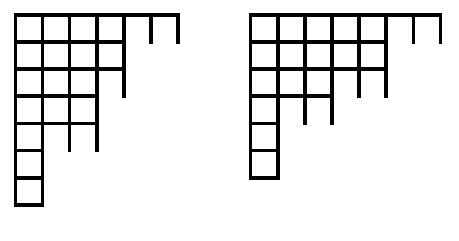
\includegraphics[width=6cm]{fig21.pdf}\\[0.3em]{\small 图 21}\end{minipage}\par\nopagebreak

现在把任一函数 $\varphi(\boldsymbol{r}_1,\boldsymbol{r}_2,\cdots,\boldsymbol{r}_N)$ 分别对每行中所填的那些变量对称化.经过这样的对称化以后，我们只能对不在同一行中的变量进行交替运算；对同一行中的一对变量进行交替运算后显然恒等于零.

在每一行中挑出一个变量，我们可以假定这些变量都在每行的第一格中，这样假定并不失其普遍性（对称化后，每行中的变量次序是无所谓的）；现在对这些变量施行交替运算.随后把第一列删去，留下的“削减”图中，再在每一行中挑出一个变量，然后对这些变量进行交替运算；这些变量又可以看作处于“削减图”的第一列.把这样的手续继续下去，我们最后得到一个函数，这个函数起先是对每行中的变量对称化的，随后又对每列中的变量进行了交替运算.经过交替运算后，一般讲来，这个函数对每行中的变量就不再对称.它只对第一行中留下的未经交替运算的那一部分变量保持着对称性，这部分变量处于第一行末端比别行突出的那些方格中.

把 $N$ 个变量用各种方式分配到一个杨图的各行中去以后（每行各格中的分配方式是无所谓的），我们就可以得到一组函数，当 $N$ 个变量以任意方式置换时\footnote{也可以按相反次序施行对称化运算和交替运算；先对每列的变量进行交替运算，再对每行的变量进行对称化运算.但这实际上不会得到新结果，用这两种方法求得的两套函数，只差一个线性变换.}，这组函数就变成它们的线性组合.但应强调指出，这些函数并不都是线性独立的；独立函数的个数往往小于 $N$ 个变量分配于该图各行中所能具有的各种分配方式的总数.我们不打算详述这一点\footnote{彼此进行线性变换的一组独立函数构成置换群的一个不可约表示的一组基，独立函数的个数就是该表示的维数.对自旋 $\frac{1}{2}$ 的粒子，这个数的推导见后面例题 1.}.

由此可见，一个杨图确定了一组具有一定的置换对称类型的函数.（对一个给定的 $N$ 值）画出所有可能的杨图，可以得到所有可能的对称类型.这相当于把 $N$ 分割成几部分之和且每部分之值小于或等于 $N$ 时，一共有多少种不同的分割方式；例如 $N=4$ 时，可能的分割方式有 $4,3+1,2+2,2+1+1,1+1+1+1$.

系统的每一个能级和一个杨图相对应，该图确定了薛定谔方程的某组解答所具有的置换对称性；一般讲来，每一个能级有若干个不同函数与之相对应，这些函数在变量的置换下彼此线性变换.这种“置换简并”的存在，是由于每个 $\hat{P}$ 算符和哈密顿量对易，但彼此不对易（见§10中段）.但是必须强调指出，这一点并不表示该能级不再具有其它的物理简并.所有这些不同的坐标波函数，乘上自旋函数以后，组合成为一个完整波函数，就可满足对称或反对称条件（由粒子的自旋决定）.

在各种类型的置换对称性（对给定的 $N$ 而言）中，总有两种类型的对称性只能分别对应于一个函数.一种对应于一个所有变量的对称函数，另一种则对应于一个反对称函数；在前一种情形下，杨图只有一行（此行有 $N$ 格），第二种情形下杨图只有一列.

现在来考虑自旋波函数 $\chi(\sigma_1,\sigma_2,\cdots,\sigma_N)$.它们对粒子置换所具有的对称类型同样由杨图给出，图中的变量现在是粒子自旋的 $z$ 分量.产生的问题是，自旋波函数的杨图应该具有怎样的形状，才能与坐标函数的一个给定杨图相配合.先设粒子的自旋具有整数值，则完整波函数 $\boldsymbol{\psi}$ 必须对所有的粒子对称.由于这一点，自旋函数和坐标函数的对称性必须由同一杨图给出，从而完整波函数 $\boldsymbol{\psi}$ 可以表成这两种函数的特定的双线性组合；在这里我们不打算详述这样的线性组合问题.

其次，设粒子的自旋为半整数值.则完整波函数必须对所有的粒子反对称.根据这一点可以证明，坐标函数的杨图和自旋函数的杨图必须具有对偶关系，亦即两者可以通过行列对调而相互得到（例如图21中的两个杨图）.

让我们对自旋为 $\frac{1}{2}$ 的重要情形（譬如对电子）进行较详细的考虑.每一个自旋变量 $\sigma_1,\sigma_2,\cdots$ 现在只取 $\pm\frac{1}{2}$ 两个值.由于一个函数对取值相同的两个任意变量反对称化后等于零，故函数 $\chi$ 只能对一对变量施行交替运算；如果对三个变量施行交替运算，其中必有两个变量取值相同，故其结果等于零.

由此可知，对一个多电子系统讲来，自旋函数的杨图中每一列只能有一格或两格（亦即此图只能有一行或两行）；对坐标函数的杨图而言，只能有一列或两列.含有 $N$ 个电子的系统中，置换对称性的类型数就等于把 $N$ 分割成为一部分或两部分之和的可能分割方式数.当 $N$ 为偶数时，这个数值等于 $\frac{1}{2}N+1$（第二部分分别为 $0,1,\cdots,\frac{1}{2}N$），当 $N$ 为奇数时它等于 $\frac{1}{2}(N+1)$（第二部分分别为 $0,1,\cdots,\frac{1}{2}(N-1)$）.例如 $N=4$ 时，所有的杨图（坐标的和自旋的）如图22所示.

容易证明，每一种对称类型（即每一杨图）对应于多电子系统的一个确定的总自旋 $S$.我们把自旋函数考虑成为旋量形式，即把它看做是一个 $N$ 秩旋量 $\chi^{\lambda\mu\cdots}$，这个旋量中的各个指标（每一个指标对应于一个单粒子的自旋）就是排列在杨图中的那些变量.我们来研究一个杨图，其第一行有 $N_1$ 格，第二行有 $N_2$ 格（$N_1+N_2=N$，及 $N_1\geqslant N_2$）.前面的 $N_2$ 列中，每列只有两格，这个旋量必须对每一列中的一对指标反对称.但是对第一行中后面剩下的 $n=N_1-N_2$ 格而言，还必须对这些格子中的变量为对称.

\par\nopagebreak\noindent\begin{minipage}{\linewidth}\centering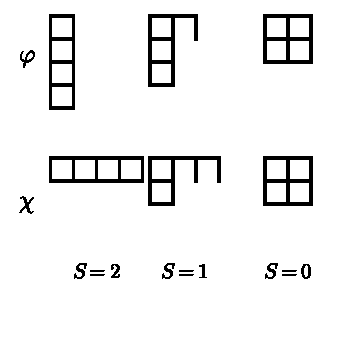
\includegraphics[width=6.5cm]{fig22.pdf}\\[0.3em]{\small 图 22}\end{minipage}\par\nopagebreak

我们知道，这样的一个 $N$ 秩旋量可以化成一个 $n$ 秩对称旋量，与总自旋 $S=\frac{1}{2}n$ 相对应.至于坐标函数的杨图，我们可以这样说，如果该图中只含一个格子的行数共有 $n$ 行，这个图就对应于总自旋 $S=\frac{1}{2}n$.当 $N$ 为偶数时，总自旋可取 0 到 $\frac{1}{2}N$ 的各种整数值，$N$ 为奇数时，可取 $\frac{1}{2}$ 到 $\frac{1}{2}N$ 的各种半整数值，这正是应有的结果.

需要强调的是，杨图与总自旋之间的这种一一对应关系，只对自旋为 $\frac{1}{2}$ 的粒子所组成的系统成立；这一点，已在上节的双粒子系统中看到.对自旋为 $s$ 的 $N$ 个粒子所组成的系统，自旋波函数由 $N$ 个 $2s$ 秩对称旋量的乘积所组成，是一个 $2Ns$ 秩的旋量.如果这个旋量按 $N$ 格的一个特定杨图进行对称化，一般讲来，可从这个对称旋量的独立分量中构造出几套线性组合，每套对应于系统的一个不同总自旋 $S$.

自旋 $\frac{1}{2}$ 粒子的自旋函数的杨图每列不能超过两格，同理，自旋为任意值 $s$ 的粒子，每列不能超过 $2s+1$ 格.

如果系统中的粒子数 $N$ 为 $2s+1$ 的整倍数，各种可能的杨图中含有一个每列为 $2s+1$ 格的矩形图.它对应于总自旋的一个定值，即 $S=0$.由此可以得出结论，如果两个（自旋）杨图能够拼成一个高为 $2s+1$ 的矩形，则两者的 $S$ 值相同\footnote{例如下列两图（对于 $s=1$）中，
\begin{center}
  \setlength{\unitlength}{1pt}%
  \begin{picture}(120,40)
    % 左图：实线杨图 (4,2,1)＋虚线补图，位于 4×3 矩形内
    \yh{0}{36}{48}\yh{0}{24}{48}\yh{0}{12}{12}\yh{0}{0}{12}%
    \yv{0}{0}{36}\yv{12}{0}{36}\yv{24}{12}{24}\yv{36}{24}{12}\yv{48}{24}{12}%
    \ydh{12}{12}{36}\ydh{12}{0}{36}\ydv{24}{0}{12}\ydv{36}{0}{24}\ydv{48}{0}{24}%
    % 右图：实线杨图 (4,3)＋虚线补图，位于 4×3 矩形内
    \yh{70}{36}{48}\yh{70}{24}{48}\yh{70}{12}{36}%
    \yv{70}{0}{36}\yv{82}{12}{24}\yv{94}{12}{24}\yv{106}{12}{24}\yv{118}{24}{12}%
    \ydh{106}{12}{12}\ydh{70}{0}{48}\ydv{82}{0}{12}\ydv{94}{0}{12}\ydv{106}{0}{12}\ydv{118}{0}{24}%
  \end{picture}
\end{center}
\noindent 实线图和虚线图是两个互补\textbf{杨图}.}.这是角动量相加法则的一个简单推论，该法则便是两个角动量只有绝对值相同时才有可能相加后得零.

作为本节的结束，让我们回到早在§20末尾附注中提及的问题，对一个全同粒子系统讲来，我们不能断言最低能量的定态波函数一定无节点.现在我们可以详述并解释其原由.

如果波函数（指坐标函数）无节点，它必须对所有粒子对称；要是它对粒子 $1,2$ 的对换为反对称，在 $\boldsymbol{r}_1=\boldsymbol{r}_2$ 处将等于零.可是，如果该系统含有 3 个或 3 个以上的电子，就不可能有全对称的坐标波函数（坐标函数的杨图每行不能超过两格）.由此可见，尽管对应于最低本征值的薛定谔方程之解是无节点的（根据变分法定理），这个解在物理上可能不允许；因而薛定谔方程的最小本征值不再对应于系统的基态，而基态波函数一般讲来将是有节点的.对于自旋为半整数 $s$ 的粒子，这种情况出现于粒子数超过 $2s+1$ 的系统中，对玻色子系统，全对称坐标波函数总是可以存在的.

\begin{xiti}

\noindent{\heiti 习题1}\quad 一个系统由 $N$ 个自旋为 $\frac{1}{2}$ 的粒子所组成，求具有不同总自旋值 $S$ 的能级总数.

解：给定了该系统的一个总自旋投影值 $M_s=\sum\sigma$ 以后，可以有 $f(M_s)$ 种不同方式给出以上的 $M_s$ 值：
\begin{equation*}
  f(M_s)=\frac{N!}{\left(\dfrac{N}{2}+M_s\right)!\left(\dfrac{N}{2}-M_s\right)!}
\end{equation*}
$f(M_s)$ 等于 $N$ 个事物中一次取出 $\frac{N}{2}+M_s$ 个事物的组合数，因为我们可令 $\frac{N}{2}+M_s$ 个粒子的 $\sigma=\frac{1}{2}$，其余粒子的 $\sigma=-\frac{1}{2}$.每一能级具有一个给定的 $S$ 值，其中共有 $2S+1$ 个不同的态，这些态的自旋投影值分别为 $M_s=S,S-1,\cdots,-S$.因此容易证明：具有给定 $S$ 值的不同能级数为
\begin{equation*}
  n(S)=f(S)-f(S+1)=\frac{N!\left(2S+1\right)}{\left(\dfrac{N}{2}+S+1\right)!\left(\dfrac{N}{2}-S\right)!}.
\end{equation*}
不同能级的总数为（当 $N$ 为偶数时）
\begin{equation*}
  n=\sum_S n(S)=f(0)=\frac{N!}{\left(\dfrac{N}{2}!\right)^2},
\end{equation*}
当 $N$ 为奇数时，则有
\begin{equation*}
  n=f\left(\frac{1}{2}\right)=\frac{N!}{\left(\dfrac{N+1}{2}\right)!\left(\dfrac{N-1}{2}\right)!}.
\end{equation*}

\noindent{\heiti 习题2}\quad 系统由自旋为 1 的粒子所组成，求各种对称类型的自旋函数所具有的总自旋值 $S$.设该系统的粒子数为 $2,3,4$.

解：对双粒子系统，这个对应关系由下列事实所确立：粒子对换后，自旋波函数应乘以 $(-1)^{2s-S}$（见§62末）.对于 $s=1$ 的粒子，由此得
\setcounter{equation}{0}\renewcommand{\theequation}{\arabic{equation}}%
\begin{equation}
  \setlength{\unitlength}{1pt}%
  \begin{picture}(140,72)
    % (a) 两格横排
    \yh{24}{60}{24}\yh{24}{72}{24}\yv{24}{60}{12}\yv{36}{60}{12}\yv{48}{60}{12}%
    \ytl{36}{56}{$S=0,2$}\ytl{36}{42}{(a)}%
    % (b) 两格竖排
    \yh{90}{48}{12}\yh{90}{60}{12}\yh{90}{72}{12}\yv{90}{48}{24}\yv{102}{48}{24}%
    \ytl{96}{44}{$S=1$}\ytl{96}{30}{(b)}%
  \end{picture}
\end{equation}
对于三粒子系统的各个杨图，可从(1)出发以各种可能的方式添加一格后获得，结果可写成下列符号式：
\begin{equation*}
\begin{gathered}
  \vcenter{\hbox{%
  \begin{picture}(24,24)
    \yh{0}{12}{24}\yh{0}{24}{24}\yv{0}{12}{12}\yv{12}{12}{12}\yv{24}{12}{12}%
    \ytl{12}{8}{$0,2$}%
  \end{picture}}}%
  \;\times\;
  \vcenter{\hbox{%
  \begin{picture}(12,24)
    \yh{0}{12}{12}\yh{0}{24}{12}\yv{0}{12}{12}\yv{12}{12}{12}%
    \ytl{6}{8}{$1$}%
  \end{picture}}}%
  \;=\;
  \underbrace{%
  \vcenter{\hbox{%
  \begin{picture}(36,24)
    \yh{0}{0}{36}\yh{0}{12}{36}\yv{0}{0}{12}\yv{12}{0}{12}\yv{24}{0}{12}\yv{36}{0}{12}%
    \ybl{18}{14}{(a)}%
  \end{picture}}}%
  \;+\;
  \vcenter{\hbox{%
  \begin{picture}(24,36)
    \yh{0}{0}{12}\yh{0}{12}{24}\yh{0}{24}{24}\yv{0}{0}{24}\yv{12}{0}{24}\yv{24}{12}{12}%
    \ybl{12}{26}{(b)}%
  \end{picture}}}}_{1,1,2,3}\\[1.6em]
  \vcenter{\hbox{%
  \begin{picture}(12,36)
    \yh{0}{12}{12}\yh{0}{24}{12}\yh{0}{36}{12}\yv{0}{12}{24}\yv{12}{12}{24}%
    \ytl{6}{8}{$1$}%
  \end{picture}}}%
  \;\times\;
  \vcenter{\hbox{%
  \begin{picture}(12,24)
    \yh{0}{12}{12}\yh{0}{24}{12}\yv{0}{12}{12}\yv{12}{12}{12}%
    \ytl{6}{8}{$1$}%
  \end{picture}}}%
  \;=\;
  \underbrace{%
  \vcenter{\hbox{%
  \begin{picture}(24,36)
    \yh{0}{0}{12}\yh{0}{12}{24}\yh{0}{24}{24}\yv{0}{0}{24}\yv{12}{0}{24}\yv{24}{12}{12}%
    \ybl{12}{26}{(b)}%
  \end{picture}}}%
  \;+\;
  \vcenter{\hbox{%
  \begin{picture}(12,48)
    \yh{0}{0}{12}\yh{0}{12}{12}\yh{0}{24}{12}\yh{0}{36}{12}\yv{0}{0}{36}\yv{12}{0}{36}%
    \ybl{6}{38}{(c)}%
  \end{picture}}}}_{0,1,2}
\end{gathered}
\end{equation*}
$S$ 值见每图下面，三粒子系统（右边的图）的总自旋值来自双粒子系统和单粒子系统（左边的图）自旋的角动量相加法则\footnote{图的右边下面有两个 1，这是由于第一个 1 来自角动量 0 和 1 的相加，第二个 1 来自角动量 2 和 1 的相加.}.式右各图的 $S$ 值的分配可以这样来建立，先注意到上图第二式图(c)（一列三格）对应于 $S=0$，故图(b)的值为剩下的 1 和 2，第一式中扣掉(b)后，知(a)的 $S$ 值为 1 和 3：
\begin{equation}
  \setlength{\unitlength}{1pt}%
  \begin{picture}(150,64)
    % (a) 三格横排
    \yh{8}{52}{36}\yh{8}{64}{36}\yv{8}{52}{12}\yv{20}{52}{12}\yv{32}{52}{12}\yv{44}{52}{12}%
    \ytl{26}{48}{$S=1,3$}\ytl{26}{34}{(a)}%
    % (b) 上二下一
    \yh{60}{40}{12}\yh{60}{52}{24}\yh{60}{64}{24}\yv{60}{40}{24}\yv{72}{40}{24}\yv{84}{52}{12}%
    \ytl{72}{36}{$S=1,2$}\ytl{72}{22}{(b)}%
    % (c) 三格竖排
    \yh{104}{28}{12}\yh{104}{40}{12}\yh{104}{52}{12}\yh{104}{64}{12}\yv{104}{28}{36}\yv{116}{28}{36}%
    \ytl{110}{24}{$S=0$}\ytl{110}{10}{(c)}%
  \end{picture}
\end{equation}
四粒子系统的杨图可在(2)基础上添加一格得到，但不能出现超过三格的列：
\begin{equation*}
\begin{gathered}
  \vcenter{\hbox{%
  \begin{picture}(36,24)
    \yh{0}{12}{36}\yh{0}{24}{36}\yv{0}{12}{12}\yv{12}{12}{12}\yv{24}{12}{12}\yv{36}{12}{12}%
    \ytl{18}{8}{$1,3$}%
  \end{picture}}}%
  \;\times\;
  \vcenter{\hbox{%
  \begin{picture}(12,24)
    \yh{0}{12}{12}\yh{0}{24}{12}\yv{0}{12}{12}\yv{12}{12}{12}%
    \ytl{6}{8}{$1$}%
  \end{picture}}}%
  \;=\;
  \underbrace{%
  \vcenter{\hbox{%
  \begin{picture}(48,24)
    \yh{0}{0}{48}\yh{0}{12}{48}\yv{0}{0}{12}\yv{12}{0}{12}\yv{24}{0}{12}\yv{36}{0}{12}\yv{48}{0}{12}%
    \ybl{24}{14}{(a)}%
  \end{picture}}}%
  \;+\;
  \vcenter{\hbox{%
  \begin{picture}(36,36)
    \yh{0}{0}{12}\yh{0}{12}{36}\yh{0}{24}{36}\yv{0}{0}{24}\yv{12}{0}{24}\yv{24}{12}{12}\yv{36}{12}{12}%
    \ybl{18}{26}{(b)}%
  \end{picture}}}}_{0,1,2,2,3,4}\\[1.6em]
  \vcenter{\hbox{%
  \begin{picture}(24,38)
    \yh{0}{14}{12}\yh{0}{26}{24}\yh{0}{38}{24}\yv{0}{14}{24}\yv{12}{14}{24}\yv{24}{26}{12}%
    \ytl{12}{10}{$1,2$}%
  \end{picture}}}%
  \;\times\;
  \vcenter{\hbox{%
  \begin{picture}(12,24)
    \yh{0}{12}{12}\yh{0}{24}{12}\yv{0}{12}{12}\yv{12}{12}{12}%
    \ytl{6}{8}{$1$}%
  \end{picture}}}%
  \;=\;
  \underbrace{%
  \vcenter{\hbox{%
  \begin{picture}(36,36)
    \yh{0}{0}{12}\yh{0}{12}{36}\yh{0}{24}{36}\yv{0}{0}{24}\yv{12}{0}{24}\yv{24}{12}{12}\yv{36}{12}{12}%
    \ybl{18}{26}{(b)}%
  \end{picture}}}%
  \;+\;
  \vcenter{\hbox{%
  \begin{picture}(24,36)
    \yh{0}{0}{24}\yh{0}{12}{24}\yh{0}{24}{24}\yv{0}{0}{24}\yv{12}{0}{24}\yv{24}{0}{24}%
    \ybl{12}{26}{(c)}%
  \end{picture}}}%
  \;+\;
  \vcenter{\hbox{%
  \begin{picture}(24,46)
    \yh{0}{0}{12}\yh{0}{12}{12}\yh{0}{24}{24}\yh{0}{36}{24}\yv{0}{0}{36}\yv{12}{0}{36}\yv{24}{24}{12}%
    \ybl{12}{38}{(d)}%
  \end{picture}}}}_{0,1,1,2,2,3}\\[1.6em]
  \vcenter{\hbox{%
  \begin{picture}(12,58)
    \yh{0}{22}{12}\yh{0}{34}{12}\yh{0}{46}{12}\yh{0}{58}{12}\yv{0}{22}{36}\yv{12}{22}{36}%
    \ytl{6}{18}{$0$}%
  \end{picture}}}%
  \;\times\;
  \vcenter{\hbox{%
  \begin{picture}(12,24)
    \yh{0}{12}{12}\yh{0}{24}{12}\yv{0}{12}{12}\yv{12}{12}{12}%
    \ytl{6}{8}{$1$}%
  \end{picture}}}%
  \;=\;
  \vcenter{\hbox{%
  \begin{picture}(24,70)
    \yh{0}{22}{12}\yh{0}{34}{12}\yh{0}{46}{24}\yh{0}{58}{24}\yv{0}{22}{36}\yv{12}{22}{36}\yv{24}{46}{12}%
    \ybl{12}{60}{(d)}\ytl{12}{18}{$1$}%
  \end{picture}}}
\end{gathered}
\end{equation*}
这里图(c)可和(1)中的(a)并成三格高的矩形，故其 $S$ 值也是 0 和 2.图(b)的 $S$ 值可从上面第二式剩下的数得到，图(a)则可从第一式剩下的 $S$ 值得到：
\begin{equation*}
  \setlength{\unitlength}{1pt}%
  \begin{picture}(230,64)
    % (a) 四格横排
    \yh{8}{52}{48}\yh{8}{64}{48}\yv{8}{52}{12}\yv{20}{52}{12}\yv{32}{52}{12}\yv{44}{52}{12}\yv{56}{52}{12}%
    \ytl{32}{48}{$S=0,2,4$}\ytl{32}{34}{(a)}%
    % (b) 上三下一
    \yh{80}{40}{12}\yh{80}{52}{36}\yh{80}{64}{36}\yv{80}{40}{24}\yv{92}{40}{24}\yv{104}{52}{12}\yv{116}{52}{12}%
    \ytl{98}{36}{$S=1,2,3$}\ytl{98}{22}{(b)}%
    % (c) 二乘二
    \yh{140}{40}{24}\yh{140}{52}{24}\yh{140}{64}{24}\yv{140}{40}{24}\yv{152}{40}{24}\yv{164}{40}{24}%
    \ytl{152}{36}{$S=0,2$}\ytl{152}{22}{(c)}%
    % (d) 上二下二（[2,1,1]）
    \yh{188}{28}{12}\yh{188}{40}{12}\yh{188}{52}{24}\yh{188}{64}{24}\yv{188}{28}{36}\yv{200}{28}{36}\yv{212}{52}{12}%
    \ytl{200}{24}{$S=1$}\ytl{200}{10}{(d)}%
  \end{picture}
\end{equation*}

\end{xiti}
\setcounter{equation}{0}\renewcommand{\theequation}{\thesection.\arabic{equation}}%

\section{二次量子化·玻色统计情形}

在大量全同粒子所组成的系统的理论中，有一种广泛使用的方法，称为二次量子化方法，这个方法在相对论理论中尤为需要，在那里述及的是粒子数可变的系统\footnote{二次量子化方法对辐射理论中的光子而言，是由 P.~A.~M. 狄拉克（1927）所发展的.随后维格纳（E.~Wigner）和约当（P.~Jordan）把它推广到费米粒子情形（1928）.}.

令 $\psi_1(\xi),\psi_2(\xi),\cdots$ 为一组完备的正交归一化的单粒子定态波函数\footnote{和 §61 一样，$\xi$ 代表粒子坐标及其自旋投影值，对 $\xi$ 积分意味着对坐标积分以及对 $\sigma$ 求和.}，它们可以是一组处于任意确定外场中的粒子态，但通常简单地取作一组平面波，也就是一组具有确定动量值（以及自旋投影值）的自由粒子波函数.为了使它成为离散态，我们考虑粒子运动于一个很大的但是有限的区域内，它的动量分量的本征值呈离散谱，相邻本征值的间距便和该区的线度成反比，并随线度的增大而趋于零.

在一个自由粒子系统中，每个粒子的动量分别守恒，因此态的占有数亦即处于 $\psi_1,\psi_2,\cdots$ 各态中的粒子数 $N_1,N_2,\cdots$ 也是守恒的.在一个相互作用的粒子系统中，每个粒子的动量并不守恒，因此占有数也不守恒.对于这样的系统，我们能考虑的只是占有数具有各种数值的概率分布.我们来寻求一种数学表述，其中以占有数（不是以粒子的坐标和自旋投影值）作为独立变量.

在这种表述中，用狄拉克符号（见§11）比较方便，用 $N_1,N_2,\cdots$ 来确定量子粒子的状态.与波函数(61.3)和(61.5)相对应的状态用 $|N_1,N_2,\cdots\rangle$ 表示.而坐标变量和自旋变量已不再明显出现.

与这种独立变量的选择相对应，各种物理量（包括系统的哈密顿量）的算符也应该改写成作用到占有数函数之上的形式.这样的表述，可以在算符的通常矩阵表示基础上得到.该算符的矩阵元必须与无相互作用粒子系统的定态波函数联系起来考虑.因为这样的态能用确定的占有数描述，能够显示出算符作用在占有数变量上的性质.

我们先来考虑遵循玻色统计的多粒子系统.设 $\hat{f}_a^{(1)}$ 是粒子 $a$ 的某个物理量算符，它只作用在 $\xi_a$ 的函数上.我们引入下列算符：
\begin{equation}
  \hat{F}^{(1)}=\sum_a\hat{f}_a^{(1)},
\end{equation}
它对所有的粒子对称（$\sum_a$ 是对所有的粒子求和），现在来求这个算符对(61.3)式波函数而言的矩阵元.首先，我们容易证明，只有 $N_1,N_2,\cdots$ 等值保持不变的跃迁矩阵元（对角矩阵元），以及其中的一个数值增加 1 另一个数值减少 1 的那些跃迁矩阵元才不等于零.因为每一个 $\hat{f}_a^{(1)}$ 算符只作用在 $\psi_{p_1}(\xi_1)\psi_{p_2}(\xi_2)\cdots\psi_{p_N}(\xi_N)$ 乘积中的一个函数上，所以不等于零的跃迁矩阵元中，只能有一个单粒子态发生改变；这就意味着某一态中的粒子数减少了一个，而在另一态中的粒子数相应地增加了一个.这类矩阵元的计算实际上很简单；读一遍不如自己算一遍.因此我们只给出计算结果.非对角矩阵元为
\begin{equation}
  \langle N_i,N_k-1|\hat{F}^{(1)}|N_i-1,N_k\rangle=f_{ik}^{(1)}\sqrt{(N_iN_k)}.
\end{equation}
为简便计，我们只写出该矩阵元的非对角下标，略去了其余的下标.式中的 $f_{ik}^{(1)}$ 为下列矩阵元：
\begin{equation}
  f_{ik}^{(1)}=\int\psi_i^{*}(\xi)\hat{f}^{(1)}\psi_k(\xi)\,\mathrm{d}\xi.
\end{equation}
要注意的是算符 $\hat{f}_a^{(1)}$（$a=1,2,\cdots$）具有完全相同的形式，只是作用在不同名称的变量上而已，所以积分 $f_{ik}^{(1)}$ 和 $a$ 无关.$F^{(1)}$ 的对角矩阵元即 $F^{(1)}$ 在 $\boldsymbol{\varPsi}_{N_1N_2\cdots}$ 态中的平均值，我们用 $\overline{F^{(1)}}$ 表示.计算后给出
\begin{equation}
  \overline{F^{(1)}}=\sum_i f_{ii}^{(1)}N_i.
\end{equation}
现在引入算符 $\hat{a}_i$，它在二次量子化方法中起着首要的作用；这个算符不是作用在坐标函数上，而是作用在 $N_1,N_2,\cdots$ 等变量上，其定义如下.算符 $\hat{a}_i$ 作用在函数 $|N_1,N_2,\cdots\rangle$ 上后，变量 $N_i$ 的数值减少 1，同时使这个波函数乘以 $\sqrt{N_i}$：
\begin{equation}
  \hat{a}_i|N_1,N_2,\cdots,N_i,\cdots\rangle=\sqrt{N_i}\,|N_1,N_2,\cdots,N_i-1,\cdots\rangle.
\end{equation}
我们可以说 $\hat{a}_i$ 算符使第 $i$ 个态的粒子数减少一个；因此称为粒子的湮没算符.可用矩阵形式表示，其不等于零的矩阵元为
\begin{equation}
  \langle N_i-1|a_i|N_i\rangle=\sqrt{N_i}.
\end{equation}
根据定义［见(11.9)式］，$\hat{a}_i$ 的厄米共轭算符 $\hat{a}_i^{+}$ 的非零矩阵元只有
\begin{equation}
  \langle N_i|a_i^{+}|N_i-1\rangle=\langle N_i-1|a_i|N_i\rangle^{*}=\sqrt{N_i}.
\end{equation}
这就表明，$\hat{a}_i^{+}$ 算符作用在 $|N_1,N_2,\cdots\rangle$ 函数上时，使 $N_i$ 的数值增加 1：
\begin{equation}
  \hat{a}_i^{+}|N_1,N_2,\cdots,N_i,\cdots\rangle=\sqrt{N_i+1}\,|N_1,N_2,\cdots,N_i+1,\cdots\rangle.
\end{equation}
换句话说，$\hat{a}_i^{+}$ 算符使第 $i$ 个态的粒子数增加一个，因此它称为粒子的产生算符.

算符乘积 $\hat{a}_i^{+}\hat{a}_i$ 作用在波函数上，所有的 $N_1,N_2,\cdots$ 变量显然都不变，而使该函数乘一常数，这是因为 $\hat{a}_i$ 算符使 $N_i$ 减少 1 但 $\hat{a}_i^{+}$ 算符又使 $N_i$ 回至原值.(64.6)和(64.7)式的两个矩阵直接相乘后，可证 $\hat{a}_i^{+}\hat{a}_i$ 的矩阵确是一个对角矩阵，并且对角矩阵元等于 $N_i$.我们可写作
\begin{equation}
  \hat{a}_i^{+}\hat{a}_i=N_i.
\end{equation}
同法可证
\begin{equation}
  \hat{a}_i\hat{a}_i^{+}=N_i+1.
\end{equation}
以上两式相减，得算符 $\hat{a}_i$ 和 $\hat{a}_i^{+}$ 的对易关系：
\begin{equation}
  \hat{a}_i\hat{a}_i^{+}-\hat{a}_i^{+}\hat{a}_i=1.
\end{equation}
$i$ 和 $k$ 不同的两算符作用在不同的变量（$N_i$ 和 $N_k$）上，是对易的：
\begin{equation}
  \hat{a}_i\hat{a}_k-\hat{a}_k\hat{a}_i=0,\quad
  \hat{a}_i\hat{a}_k^{+}-\hat{a}_k^{+}\hat{a}_i=0\quad(i\neq k).
\end{equation}
根据算符 $\hat{a}_i,\hat{a}_i^{+}$ 的上述性质，易证下列算符
\begin{equation}
  \hat{F}^{(1)}=\sum_{i,k}f_{ik}^{(1)}\hat{a}_i^{+}\hat{a}_k
\end{equation}
与(64.1)式的算符相同.因为按(64.6)，(64.7)算出的所有矩阵元等于(64.2)，(64.4)中的矩阵元.这是一个非常重要的结果.(64.13)式中的 $f_{ik}^{(1)}$ 不过是一些数值.因此，我们可以把作用于坐标函数上的一个普通算符表为作用于新变量占有数 $N_i$ 函数上的算符.

以上所得的结果，很容易推广到其它形式的算符上.令
\begin{equation}
  \hat{F}^{(2)}=\sum_{a>b}\hat{f}_{ab}^{(2)},
\end{equation}
其中的 $\hat{f}_{ab}^{(2)}$ 为同时属于两个粒子的一个物理量算符，因而作用在 $\xi_a$ 及 $\xi_b$ 的函数上.同样的计算表明，这个算符可以通过 $\hat{a}_i,\hat{a}_i^{+}$ 算符表为
\begin{equation}
  \hat{F}^{(2)}=\frac{1}{2}\sum_{i,k,l,m}\langle ik|\,f^{(2)}\,|lm\rangle\,\hat{a}_i^{+}\hat{a}_k^{+}\hat{a}_m\hat{a}_l,
\end{equation}
其中
\begin{equation*}
  \langle ik|\,\hat{f}^{(2)}\,|lm\rangle=\iint\psi_i^{*}(\xi_1)\psi_k^{*}(\xi_2)\hat{f}^{(2)}\psi_l(\xi_1)\psi_m(\xi_2)\,\mathrm{d}\xi_1\mathrm{d}\xi_2.
\end{equation*}
这几个公式显然可以推广到对所有粒子对称的其它任意形式的算符上（例如 $\hat{F}^{(3)}=\sum\hat{f}_{abc}^{(3)}$ 这些形式，等等）.

通过这些公式，可用算符 $\hat{a}_i$ 和 $\hat{a}_i^{+}$ 表达出具有 $N$ 个相互作用全同粒子的物理系统的哈密顿量.这种系统的哈密顿量对所有的粒子当然是对称的.在非相对论近似下\footnote{不存在磁场时.}，可表成下列一般形式：
\begin{equation}
\begin{aligned}
  \hat{H}={}&\sum_a\hat{H}_a^{(1)}+\sum_{a>b}U^{(2)}(\boldsymbol{r}_a,\boldsymbol{r}_b)+{}\\
  &+\sum_{a>b>c}U^{(3)}(\boldsymbol{r}_a,\boldsymbol{r}_b,\boldsymbol{r}_c)+\cdots,
\end{aligned}
\end{equation}
其中的 $\hat{H}_a^{(1)}$ 为哈密顿量中只依赖于第 $a$ 个粒子坐标的算符：
\begin{equation}
  \hat{H}_a^{(1)}=-\left(\hbar^2/2m\right)\nabla_a^2+U^{(1)}(\boldsymbol{r}_a),
\end{equation}
其中的 $U^{(1)}(\boldsymbol{r}_a)$ 为一个单粒子在外场中的势能.(64.16)式中的其余部分为粒子间的相互作用能量；把它分成与两个、三个等粒子的坐标有关的项.

哈密顿量的上述表式使我们可以直接应用(64.13)，(64.15)以及类似的式子.得
\begin{equation}
  \hat{H}=\sum_{i,k}H_{ik}^{(1)}\hat{a}_i^{+}\hat{a}_k+\frac{1}{2}\sum_{i,k,l,m}\langle ik|\,U^{(2)}\,|lm\rangle\hat{a}_i^{+}\hat{a}_k^{+}\hat{a}_m\hat{a}_l+\cdots.
\end{equation}
这就是欲求的哈密顿量表式，这个算符作用在占有数的函数上.

对无相互作用的多粒子系统讲来，(64.18)式中只留下第一项：
\begin{equation}
  \hat{H}=\sum_{i,k}H_{ik}^{(1)}\hat{a}_i^{+}\hat{a}_k.
\end{equation}
如取 $\psi_i$ 为单粒子哈密顿量 $\hat{H}^{(1)}$ 的本征函数，则矩阵 $H_{ik}^{(1)}$ 是一个对角矩阵，对角元等于该粒子诸能量本征值 $\varepsilon_i$.故
\begin{equation*}
  \hat{H}=\sum_i\varepsilon_i\hat{a}_i^{+}\hat{a}_i;
\end{equation*}
$\hat{a}_i^{+}\hat{a}_i$ 算符用(64.9)式的本征值代入，可得系统能级表式
\begin{equation*}
  E=\sum_i\varepsilon_iN_i,
\end{equation*}
这是可以预料的明显结果.

引入下列 $\hat{\psi}$ 算符，可使我们所作的表述更为精练\footnote{注意(64.20)与下式的相似性：
\begin{equation*}
  \boldsymbol{\psi}=\sum_i a_i\psi_i,
\end{equation*}
这是任意波函数展为完备函数组.现在又被量子化了一次，术语二次量子化方法一词即源出于此.}：
\begin{equation}
  \hat{\psi}(\xi)=\sum_i\psi_i(\xi)\hat{a}_i,\qquad
  \hat{\psi}^{+}(\xi)=\sum_i\psi_i^{*}(\xi)\hat{a}_i^{+},
\end{equation}
其中的变量 $\xi$ 可以看作参量.根据以上所述的算符 $\hat{a}_i,\hat{a}_i^{+}$，可知算符 $\hat{\psi}$ 使该系统的粒子总数减少一个，算符 $\hat{\psi}^{+}$ 则使它增加一个.

容易证明算符 $\hat{\psi}^{+}(\xi_0)$ 在 $\xi_0$ 点处产生一个粒子.因为算符 $\hat{a}_i^{+}$ 的作用结果，是产生一个处于 $\psi_i(\xi)$ 态中的粒子.根据这一点，算符 $\hat{\psi}^{+}(\xi_0)$ 的作用结果，是产生一个状态波函数\footnote{$\delta(\xi-\xi_0)$ 是下列乘积的简写
\begin{equation*}
  \delta(x-x_0)\delta(y-y_0)\delta(z-z_0)\delta\sigma\sigma_0.
\end{equation*}}为 $\sum_i\psi_i^{*}(\xi)\psi_i(\xi_0)=\delta(\xi-\xi_0)$ 的粒子［根据公式(5.12)］，这个粒子具有确定的坐标值（和确定的自旋值）.

算符 $\hat{\psi}$ 的对易关系可根据 $\hat{a}_i,\hat{a}_i^{+}$ 的关系立刻求得：
\begin{equation}
  \hat{\psi}(\xi)\hat{\psi}(\xi')-\hat{\psi}(\xi')\hat{\psi}(\xi)=0,
\end{equation}
\begin{equation}
  \hat{\psi}(\xi)\hat{\psi}^{+}(\xi')-\hat{\psi}^{+}(\xi')\hat{\psi}(\xi)=\sum_i\psi_i(\xi)\psi_i^{*}(\xi')=\delta(\xi-\xi').
\end{equation}
二次量子化算符 $\hat{F}^{(1)}$ 可用算符 $\hat{\psi}$ 表成
\begin{equation}
  \hat{F}^{(1)}=\int\hat{\psi}^{+}(\xi)\hat{f}^{(1)}\hat{\psi}(\xi)\,\mathrm{d}\xi,
\end{equation}
其中的算符 $\hat{f}^{(1)}$ 应该理解为作用在 $\hat{\psi}(\xi)$ 中含有参量 $\xi$ 的函数上.这是因为如把(64.20)的 $\hat{\psi}$ 和 $\hat{\psi}^{+}$ 代入上式并用定义(64.3)，我们又回到(64.13)式.同样，(64.15)式变成
\begin{equation}
  \hat{F}^{(2)}=\frac{1}{2}\iint\hat{\psi}^{+}(\xi)\hat{\psi}^{+}(\xi')\hat{f}^{(2)}\hat{\psi}(\xi')\hat{\psi}(\xi)\,\mathrm{d}\xi\mathrm{d}\xi'.
\end{equation}
特别是，系统的哈密顿量可用算符 $\hat{\psi}$ 表成
\begin{equation}
\begin{aligned}
  \hat{H}={}&\int\left\{-\frac{\hbar^2}{2m}\hat{\psi}^{+}(\xi)\nabla^2\hat{\psi}(\xi)
  +\hat{\psi}^{+}(\xi)U^{(1)}(\xi)\hat{\psi}(\xi)\right\}\mathrm{d}\xi+{}\\
  &+\frac{1}{2}\iint\hat{\psi}^{+}(\xi')\hat{\psi}^{+}(\xi)U^{(2)}(\xi,\xi')\hat{\psi}(\xi')\hat{\psi}(\xi)\,\mathrm{d}\xi\mathrm{d}\xi'+\cdots.
\end{aligned}
\end{equation}
仿效粒子处于 $\psi$ 态的概率密度式 $\psi^{*}\psi$，由算符 $\hat{\psi}$ 组成的 $\hat{\psi}^{+}(\xi)\hat{\psi}(\xi)$ 算符，称为粒子密度算符.下列积分
\begin{equation}
  \hat{N}=\int\hat{\psi}^{+}\hat{\psi}\,\mathrm{d}\xi
\end{equation}
在二次量子化表述中代表系统的粒子总数算符.这是因为，把(64.20)式的算符 $\hat{\psi}$ 代入，并应用波函数的正交归一化性质，可得
\begin{equation*}
  \hat{N}=\sum\hat{a}_i^{+}\hat{a}_i.
\end{equation*}
式中的每一项代表第 $i$ 个态中的粒子数算符；根据(64.9)式，其本征值等于占有数 $N_i$，对所有的 $N_i$ 求和后，就是系统中的粒子总数\footnote{对一个具有给定粒子数的系统讲来，这个论述是自明的，这是自由粒子系统哈密顿量(64.19)式的一种性质，但推广到相对论理论中时，会产生新的不再自明的结果（参考第四卷，§11）.}.

最后，如果系统是由几类不同的玻色子组成的，二次量子化方法中必须对每类粒子定义出 $\hat{a}$ 和 $\hat{a}^{+}$ 算符.属于不同类别的粒子算符显然是对易的.

\section{二次量子化·费米统计情形}

对服从费米统计的全同粒子所组成的多粒子系统而言，二次量子化方法的基本理论全部保持不变，但是 $\hat{a}_i$ 算符以及物理量的矩阵元公式自然有所不同.

$\boldsymbol{\varPsi}_{N_1N_2\cdots}$ 波函数现在呈(61.5)形式.由于这个函数的反对称性，首先就产生了正负号问题.这个问题在玻色统计情形是没有的，因为上节的波函数是对称波函数，它的符号一旦选定后，对粒子的所有置换均保持不变.为了确定(61.5)式函数的符号起见，我们规定以下的选择方法.我们把所有的 $\psi_i$ 态编好号码.然后令(61.5)行列式中的各行按以下次序排列：
\begin{equation}
  p_1<p_2<p_3<\cdots<p_N,
\end{equation}
这个行列式中的各列依次为 $\xi_1,\xi_2,\cdots,\xi_N$ 等不同变量的函数.$p_1,p_2,\cdots,p_N$ 中不能有两个数值相同，不然，该行列式将等于零.换句话说，占有数 $N_i$ 的取值只能是零或 1.

我们再来考虑(64.1)形式的算符 $\hat{F}^{(1)}=\sum_a\hat{f}_a^{(1)}$.和§64中的情形一样，只有保持所有占有数不变的那些跃迁矩阵元，以及使一个占有数（$N_i$）减少一（从 1 变到零）另一个占有数（$N_k$）增加一（从零变到 1）的那些跃迁矩阵元才不等于零.$i<k$ 时，容易求得
\begin{equation}
  \langle 1_i,0_k|\hat{F}^{(1)}|0_i,1_k\rangle=f_{ik}^{(1)}(-1)^{\Sigma(i+1,k-1)},
\end{equation}
其中 $0_i,1_i$ 代表 $N_i=0,N_i=1$.令符号 $\Sigma(k,l)$ 代表第 $k$ 个态到第 $l$ 个态的所有占有数之和\footnote{$i>k$ 时，(65.2)式的幂次为 $\Sigma(k+1,i-1)$，但当 $i=k\pm1$ 时，这个和式应令它等于零.}：
\begin{equation*}
  \Sigma(k,l)=\sum_{n=k}^{l}N_n.
\end{equation*}
至于对角矩阵元，求得的结果就是以前的(64.4)式：
\begin{equation}
  \overline{F^{(1)}}=\sum_i f_{ii}^{(1)}N_i.
\end{equation}
为了把算符 $\hat{F}^{(1)}$ 表成(64.13)形式，算符 $\hat{a}_i$ 必须按下列矩阵元来定义：
\begin{equation}
  \langle 0_i|a_i|1_i\rangle=\langle 1_i|a_i^{+}|0_i\rangle=(-1)^{\Sigma(1,i-1)},
\end{equation}
以上两个矩阵相乘，当 $k>i$ 时可得
\begin{equation*}
\begin{aligned}
  &\langle 1_i,0_k|\,a_i^{+}a_k\,|0_i,1_k\rangle
  =\langle 1_i,0_k|\,a_i^{+}\,|0_i,0_k\rangle\langle 0_i,0_k|\,a_k\,|0_i,1_k\rangle=\\
  &=(-1)^{\Sigma(1,i-1)}(-1)^{\Sigma(1,i-1)+\Sigma(i+1,k-1)},
\end{aligned}
\end{equation*}
或
\begin{equation}
  \langle 1_i,0_k|\,a_i^{+}a_k\,|0_i,1_k\rangle=(-1)^{\Sigma(i+1,k-1)}.
\end{equation}
如果 $i=k$，$\hat{a}_i^{+}\hat{a}_i$ 矩阵为对角矩阵，它的矩阵元当 $N_i=1$ 时等于 1，当 $N_i=0$ 时等于零；因此，可写成
\begin{equation}
  \hat{a}_i^{+}\hat{a}_i=N_i.
\end{equation}
将以上两式代入(64.13)式，确实得出(65.2)，(65.3)式.

将 $\hat{a}_i^{+},\hat{a}_k$ 按相反次序相乘，便得
\begin{equation*}
\begin{aligned}
  &\langle 1_i,0_k|\,a_ka_i^{+}\,|0_i,1_k\rangle
  =\langle 1_i,0_k|\,a_k\,|1_i,1_k\rangle\langle 1_i,1_k|\,a_i^{+}\,|0_i,1_k\rangle=\\
  &=(-1)^{\Sigma(1,i-1)+\Sigma(i+1,k-1)+\Sigma(1,i-1)+1}
\end{aligned}
\end{equation*}
或
\begin{equation}
  \langle 1_i,0_k|\,a_ka_i^{+}\,|0_i,1_k\rangle=-(-1)^{\Sigma(i+1,k-1)}.
\end{equation}
与(65.7)和(65.5)比较，可知两式右边符号相反，即
\begin{equation*}
  \hat{a}_i^{+}\hat{a}_k+\hat{a}_k\hat{a}_i^{+}=0,\qquad i\neq k.
\end{equation*}
对于对角矩阵 $\hat{a}_i\hat{a}_i^{+}$，我们求得
\begin{equation}
  \hat{a}_i\hat{a}_i^{+}=1-N_i,
\end{equation}
此式与(65.6)式相加，得
\begin{equation*}
  \hat{a}_i\hat{a}_i^{+}+\hat{a}_i^{+}\hat{a}_i=1.
\end{equation*}
以上两式可合并写成
\begin{equation}
  \hat{a}_i\hat{a}_k^{+}+\hat{a}_k^{+}\hat{a}_i=\delta_{ik}.
\end{equation}
经过同样的计算，可证 $\hat{a}_i\hat{a}_k$ 乘积满足下列关系式：
\begin{equation}
  \hat{a}_i\hat{a}_k+\hat{a}_k\hat{a}_i=0
\end{equation}
（特别有 $\hat{a}_i\hat{a}_i=0$）.

由此可见，$i\neq k$ 时，$\hat{a}_i$ 和 $\hat{a}_k$（或 $\hat{a}_k^{+}$）算符反对易，而在玻色统计情形，这两个算符彼此对易.这种差别是十分自然的.在玻色统计情形下，算符 $\hat{a}_i$ 和 $\hat{a}_k$ 是完全独立的；每一个算符 $\hat{a}_i$ 只作用在一个单独的变量 $N_i$ 上，作用的结果并不依赖于其它占有数的数值.但在费米统计情形下，根据(65.4)式的定义，算符 $\hat{a}_i$ 作用的结果不但与 $N_i$ 本身有关，并且和该态之前的所有占有数有关.因此，各个算符 $\hat{a}_i,\hat{a}_k$ 的作用不能认为是彼此独立的.

算符 $\hat{a}_i$ 和 $\hat{a}_i^{+}$ 的性质如此定义以后，留下的(64.13)到(64.18)的所有其它公式全部保持不变.用(64.20)式定义的算符 $\hat{\psi}$ 表出的物理量算符的(64.23)到(64.25)各式，也都很好地成立.但是(64.21)，(64.22)式中的对易关系，现在要改成
\begin{equation}
  \hat{\psi}^{+}(\xi')\hat{\psi}(\xi)+\hat{\psi}(\xi)\hat{\psi}^{+}(\xi')=\delta(\xi-\xi'),
\end{equation}
\begin{equation}
  \hat{\psi}(\xi')\hat{\psi}(\xi)+\hat{\psi}(\xi)\hat{\psi}(\xi')=0.
\end{equation}
如果系统由两类粒子所组成，则对每类粒子可以引进它的二次量子化算符（已在上节之末提过）.玻色子算符和费米子算符彼此对易.至于异类费米子的算符，则在非相对论的理论范围内可以假定或则对易或则反对易；这两种假定，在二次量子化方法中得出同一结果.

但在相对论理论中，不同的粒子可以进行相互转变，为了今后在该理论中的应用起见，我们就应假定不同费米子的产生算符和湮没算符相互反对易.如果把同一复合粒子的两个不同内态看作两个“不同”粒子，这个假定就变得很明显.
